\Opensolutionfile{ans}[ans/CD3/Muc_5_6]
\section{Mức độ 5,6 điểm}
\begin{dang}{Xác định giá trị lớn nhất - giá trị nhỏ nhất của hàm số thông qua đồ thị, bảng biến thiên}
\end{dang}
\setcounter{ex}{0}
\setcounter{dang}{0}
\begin{ex}%[2D1Y3-1]
	[Đề tham khảo 2019]
	\immini{
	Cho hàm số $y=f(x)$ liên tục trên đoạn $[-1;3]$ và có đồ thị như hình bên. Gọi $M$ và $m$ lần lượt là giá trị lớn nhất và giá trị nhỏ nhất của hàm số đã cho trên đoạn $[-1;3]$. Giá trị của $M-m$ bằng
	\choice
	{$1$}
	{$4$}
	{\True $5$}
	{$0$}
	}{
		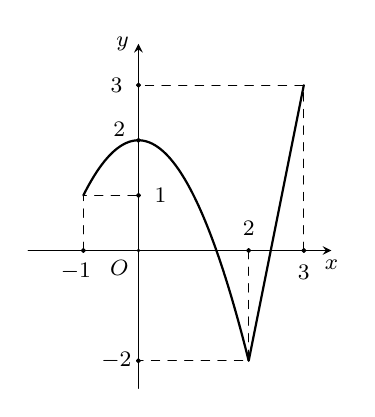
\begin{tikzpicture}[>=stealth,line join=round,line cap=round,font=\footnotesize,scale=0.7]
			\draw[->] (-2,0)--(3.5,0) node[below]{$x$};
			\draw[->] (0,-2.5)--(0,3.75) node[left]{$y$};
			\fill[name=O] (0,0) circle (1pt) node[below left] {$O$}; 
			\draw[thick,color=black, smooth, samples=100, domain= -1:2] plot(\x,{-(\x)^2 +2}) node[left]{$ $};
			\draw[thick] (2,-2)--(3,3);
			\draw[dashed] (-1,0)|-(0,1) (2,0)|-(0,-2) (3,0)|-(0,3);
			\foreach \d/\g/\l in {{-1,0}/-110/-1,{2,0}/90/2,{3,0}/-90/3,{0,-2}/180/-2,{0,1}/0/1,{0,2}/150/2,{0,3}/180/3}
			\draw[fill=black] (\d) circle (1pt) +(\g:.4) node{$\l$};
		\end{tikzpicture}
	}
	\loigiai{
		Từ đồ thị, ta có $M=\max\limits_{[-1;3]}f(x)=3$ và $m=\min\limits_{[-1;3]}f(x)=-2$.\\
		Vậy $M-m=5$.
	}
\end{ex}

%Câu 2
\begin{ex}%[2D1Y3-1]
	[Đề minh họa 2017]
	Cho hàm số $f(x)$ xác định, liên tục trên $\mathbb{R}$ và có bảng biến thiên như hình. 
	\begin{center}
		
\begin{tikzpicture}
			\tkzTabInit[nocadre=false,lgt=1.2,espcl=2,deltacl=.6]
			{$x$/0.6,$y'$/0.6,$y$/2}
			{$-\infty$,$0$,$1$,$+\infty$}
			\tkzTabLine{,+,d,-,0,+,}
			\tkzTabVar{-/$-\infty$,+/$0$,-/$-1$,+/$+\infty$}
		\end{tikzpicture}
	\end{center}
	Khẳng định nào sau đây là khẳng định đúng?
	\choice
	{Hàm số có giá trị cực tiểu bằng $1$}
	{Hàm số có giá trị lớn nhất bằng $0$ và giá trị nhỏ nhất bằng $-1$}
	{Hàm số đạt cực đại tại $x=0$ và đạt cực tiểu tại $x=1$}
	{Hàm số có đúng một cực trị}
	\loigiai{
		Từ bảng biến thiên, ta có hàm số đạt cực đại tại $x=0$ và đạt cực tiểu tại $x=1$.		
	}
\end{ex}

%Câu 3
\begin{ex}%[2D1Y3-1]
	\immini{
	Cho hàm số $y=f(x)$ liên tục trên đoạn $[-1;1]$ và có đồ thị như hình vẽ. Gọi $M$ và $m$ lần lượt là giá trị lớn nhất và giá trị nhỏ nhất của hàm số đã cho trên đoạn $[-1;1]$. Giá trị của $M-m$ bằng
	\choice
	{$0$}
	{\True $1$}
	{$2$}
	{$3$}}
	{
		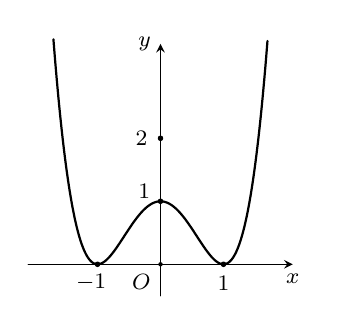
\begin{tikzpicture}[>=stealth,line join=round,line cap=round,font=\footnotesize,scale=0.8]
			\draw[->] (-2.1,0)--(2.1,0) node[below]{$x$};
			\draw[->] (0,-0.5)--(0,3.5) node[left]{$y$};
			\fill[name=O] (0,0) circle (1pt) node[below left] {$O$}; 
			\draw[thick,color=black, smooth, samples=200, domain= -1.7:1.7] plot(\x,{(\x)^4-2*(\x)^2 +1}) node[left]{$ $};
			\foreach \d/\g/\l in {{-1,0}/-110/-1,{1,0}/-90/1,{0,1}/150/1,{0,2}/180/2}
					\draw[fill=black] (\d) circle (1pt) +(\g:.3) node{$\l$};
		\end{tikzpicture}
	}
	\loigiai{
		Từ đồ thị, ta thấy $M=\max\limits_{[-1;1]}f(x)=1$ và $m=\min\limits_{[-1;1]}f(x)=0$.\\
		Vậy $M-m = 1$.	
	}
\end{ex}

%Câu 4
\begin{ex}%[2D1Y3-1]
	Cho hàm số $y=f(x)$ liên tục trên $[-3;2]$ và có bảng biến thiên như hình. 
	\begin{center}
		
\begin{tikzpicture}
			\tkzTabInit[nocadre=false,lgt=1.2,espcl=2,deltacl=.6]
			{$x$/0.6,$y$/2}
			{$-3$,$-1$,$0$,$1$,$2$}
			\tkzTabVar{-/$-2$,+/$3$,-/$0$,+/$2$,-/$1$}
		\end{tikzpicture}
	\end{center}
	Gọi $M$ và $m$ lần lượt là giá trị lớn nhất và giá trị nhỏ nhất của hàm số trên đoạn $[-1;2]$. Tính $M+m$.
	\choice
	{\True $3$}
	{$2$}
	{$1$}
	{$4$}
	\loigiai{
		Từ bảng biến thiên, ta thấy $M=\max\limits_{[-1;2]}f(x)=3$ và $m=\min\limits_{[-1;2]}f(x)=0$.\\
		Vậy $M+m=3$.
	}
\end{ex}

%Câu 5
\begin{ex}%[2D1Y3-1]
	[Chuyên Lương Thế Vinh - Đồng Nai 2019]
	\immini{Cho hàm số $y=f(x)$ xác định và liên tục trên $\mathbb{R}$ có đồ thị như hình vẽ bên. Tìm giá trị nhỏ nhất $m$ và giá trị lớn nhất $M$ của hàm số $y=f(x)$ trên đoạn $[-2;2]$.
	\choice
	{\True $m=-5$; $M=-1$}
	{$m=-2$; $M=2$}
	{$m=-1$; $M=0$}
	{$m=-5$; $M=0$}
	}{
		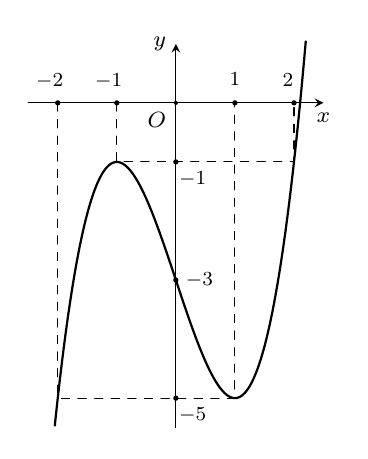
\begin{tikzpicture}[>=stealth,line join=round,line cap=round,font=\footnotesize,scale=0.75]
			\draw[->] (-2.5,0)--(2.5,0) node[below]{$x$};
			\draw[->] (0,-5.5)--(0,1) node[left]{$y$};
			\fill[name=O] (0,0) circle (1pt) node[below left] {$O$}; 
			\draw[thick,color=black, smooth, samples=100, domain= -2.05:2.2] plot(\x,{(\x)^3-3*(\x)-3}) node[left]{$ $};
			\foreach \d/\g/\l in {{-2,0}/110/-2,{-1,0}/110/-1,{1,0}/90/1,{2,0}/105/2,{0,-5}/-45/-5,{0,-3}/0/-3,{0,-1}/-45/-1}
				\draw[fill=black] (\d) circle (1pt) +(\g:.4) node[scale=0.9]{$\l$};
			\draw[dashed] (-2,0)|-(0,-5)-|(1,0) (-1,0)|-(0,-1)-|(2,0);
		\end{tikzpicture}
	}
	\loigiai{
		Từ đồ thị, ta thấy $M=\max\limits_{[-2;2]}f(x)=-1$ và $m=\min\limits_{[-2;2]}f(x)=-5$.\\
	}
\end{ex}

%Câu 6
\begin{ex}%[2D1Y3-1]
	[THPT Ba Đình 2019]
	Xét hàm số $y=f(x)$ với $x\in [-1;5]$ có bảng biến thiên như sau
	\begin{center}
		
\begin{tikzpicture}
			\tkzTabInit[nocadre=false,lgt=1.2,espcl=2,deltacl=.6]
			{$x$/0.6,$y'$/0.6,$y$/2}
			{$-1$,$0$,$2$,$5$}
			\tkzTabLine{,+,0,-,0,+,}
			\tkzTabVar{-/$3$,+/$4$,-/$0$,+/$+\infty$}
		\end{tikzpicture}
	\end{center}
	Khẳng định nào sau đây đúng?
	\choice
	{\True Hàm số đã cho không tồn tại giá trị lớn nhất trên đoạn $[-1;5]$}
	{Hàm số đã cho đạt giá trị nhỏ nhất tại $x=-1$ và $x=2$ trên đoạn $[-1;5]$}
	{Hàm số đã cho đạt giá trị nhỏ nhất tại $x=-1$ và đạt giá trị lớn nhất tại $x=-5$ trên đoạn $[-1;5]$}
	{Hàm số đã cho đạt giá trị nhỏ nhất tại $x=0$ trên đoạn $[-1;5]$}
	\loigiai{
		Từ bảng biến thiên, ta có hàm số không tồn tại giá trị lớn nhất trên đoạn $[-1;5]$.
	}
\end{ex}

%Câu 7
\begin{ex}%[2D1B3-1]
	[THPT Ba Đình 2019]
	Xét hàm số $y=f(x)$ liên tục trên $\mathbb{R}$, có bảng biến thiên như hình
	\begin{center}
		
\begin{tikzpicture}
			\tkzTabInit[nocadre=false,lgt=1.2,espcl=2,deltacl=.6]
			{$x$/0.6,$y'$/0.6,$y$/2}
			{$-\infty$,$-1$,$1$,$2$,$+\infty$}
			\tkzTabLine{,-,d,+,0,+,d,-,}
			\tkzTabVar{+/$+\infty$, -/$-3$,R,+/$2$,-/$-4$}
		\end{tikzpicture}
	\end{center}
	Trong các mệnh đề sau, mệnh đề nào {\bf sai}?
	\choice
	{Hàm số có hai điểm cực trị}
	{\True Hàm số có giá trị lớn nhất bằng $2$ và giá trị nhỏ nhất bằng $-3$}
	{Đồ thị hàm số có đúng một đường tiệm cận}
	{Hàm số nghịch biến trên mỗi khoảng $(-\infty;-1)$, $(2;+\infty)$}
	\loigiai{
		Từ bảng biến thiên,ta có
		\begin{itemize}
			\item Hàm số có hai điểm cực trị, đạt tại $x=-1$ và $x=2$.
			\item Hàm số không có giá trị lớn nhất và không có giá trị nhỏ nhất.
			\item Đồ thị hàm số có đúng một đường tiệm cận là tiệm cận ngang có phương trình $y=-4$.
			\item Hàm số nghịch biến trên mỗi khoảng $(-\infty;-1)$ và $(2;+\infty)$.
		\end{itemize}
	}
\end{ex}

%Câu 8
\begin{ex}%[2D1Y3-1]
	[Chuyên Nguyễn Tất Thành - Yên Bái 2019]
	Cho hàm số $y=f(x)$ liên tục và có bảng biến thiên trên đoạn $[-1;3]$ như hình. 
	\begin{center}
		
\begin{tikzpicture}
			\tkzTabInit[nocadre=false,lgt=1.2,espcl=2,deltacl=.6]
			{$x$/0.6,$y'$/0.6,$y$/2}
			{$-1$,$0$,$2$,$3$}
			\tkzTabLine{,+,0,-,0,+,}
			\tkzTabVar{-/$0$,+/$5$,-/$1$,+/$4$}
		\end{tikzpicture}
	\end{center}
	Khẳng định nào sau đây là đúng?
	\choice
	{\True $\max\limits_{[-1;3]}f(x) = f(0)$}
	{$\max\limits_{[-1;3]}f(x) = f(3)$}
	{$\max\limits_{[-1;3]}f(x) = f(2)$}
	{$\max\limits_{[-1;3]}f(x) = f(-1)$}
	\loigiai{
		Từ bảng biến thiên, ta có $\max\limits_{[-1;3]}f(x)=f(0)=5$.
	}
\end{ex}

%Câu 9
\begin{ex}%[2D1Y3-1]
	[VTED 2019]
	\immini{
	Cho hàm số $f(x)$ liên tục trên $[-1;5]$ và có đồ thị trên đoạn $[-1;5]$ như hình vẽ. Tổng giá trị lớn nhất và giá trị nhỏ nhất của hàm số $f(x)$ trên đoạn $[-1;5]$ bằng
	\choice
	{$-1$}
	{$4$}
	{\True $1$}
	{$2$}}
	{
		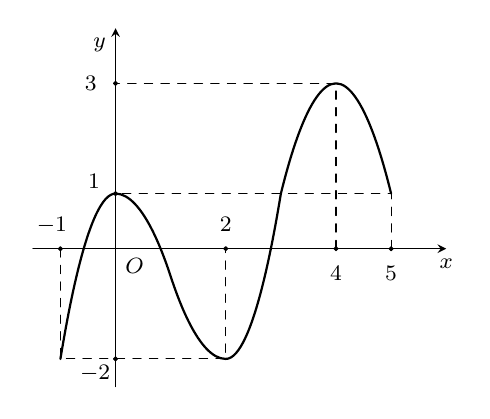
\begin{tikzpicture}[>=stealth,line join=round,line cap=round,font=\footnotesize,scale=0.7]
			\draw[->] (-1.5,0) -- (6,0) node[below] {$x$};
			\draw[->] (0,-2.5) -- (0,4) node[below left] {$y$};
			\draw(0,0) node[below right] {$O$};
			
			\draw[thick]
				(-1,-2) parabola bend (0,1) (1,-0.5)
				(1,-0.5) parabola bend (2,-2) (3,1)
				(3,1) parabola bend (4,3) (5,1)
			;
			\draw[dashed] (-1,0)|-(0,-2)-|(2,0) (5,0)|-(0,1) (4,0)|-(0,3);
			\foreach \d/\g/\l in {{-1,0}/110/-1,{2,0}/90/2,{4,0}/-90/4,{5,0}/-90/5,{0,-2}/-1
			45/-2,{0,1}/150/1,{0,3}/180/3}
				\draw[fill=black] (\d) circle (1pt) +(\g:.45) node{$\l$};
		\end{tikzpicture}
	}
	\loigiai{
		Từ đồ thị, ta có $\max\limits_{[-1;5]}f(x) + \min\limits_{[-1;5]}f(x)= 3 + (-2)=1$.
	}
\end{ex}

%Câu 10
\begin{ex}%[2D1Y3-1]
	[THPT Yên Mỹ - Hưng Yên  2019]
	\immini{
	Cho hàm số $y=f(x)$ xác định, liên tục trên $\left[-1;\dfrac{5}{2}\right]$ và có đồ thị là đường cong như hình vẽ. Giá trị lớn nhất $M$ và giá trị nhỏ nhất $m$ của hàm số $f(x)$ trên $\left[-1;\dfrac{5}{2}\right]$ là
	\choice
	{$M=4$; $m=1$}
	{\True $M=4$; $m=-1$}
	{$M=\dfrac{7}{2}$; $m=-1$}
	{$M=\dfrac{7}{2}$; $m=1$}
	}{
		\begin{tikzpicture}[>=stealth,line join=round,line cap=round,font=\footnotesize,scale=0.7]
			\draw[->] (-1.5,0) -- (3,0) node[below] {$x$};
			\draw[->] (0,-1.5) -- (0,5) node[below left] {$y$};
			\draw(0,0) node[below right,scale=0.8] {$O$};
			
			\draw[thick]
				(-1,1) parabola bend (0,3.5) (1.15,0)
				(1.15,0) parabola bend (1.6,-1) (2.5,4)
			;
			\draw[dashed] (-1,0)|-(0,1) (1.6,0)|-(0,-1) (2.5,0)|-(0,4);
			\foreach \d/\g/\l in {{-1,0}/-110/-1,{1,0}/-90/,{2,0}/90/,{3,0}/180/,{2.5,0}/-90/\tfrac{5}{2},{0,-1}/180/-1,{0,1}/0/1,{0,2}/180/,{0,3}/180/,{0,4}/180/4}
				\draw[fill=black] (\d) circle (1pt) +(\g:.45) node{$\l$};
		\end{tikzpicture}
	}
	\loigiai{
		Từ đồ thị, ta có $M=\max\limits_{\left[-1;\tfrac{5}{2}\right]}f(x)=4$ và $m=\min\limits_{\left[-1;\tfrac{5}{2}\right]}f(x)=-1$.
	}
\end{ex}

%Câu 11
\begin{ex}%[2D1Y3-1]
	[THPT Nghĩa Hưng - Nam Định 2019]
	\immini{
	Cho hàm số $y=f(x)$ có đồ thị như hình vẽ. Giá trị lớn nhất của hàm số $f(x)$ trên đoạn $[0;2]$ là
	\choice
	{$\max\limits_{[0;2]}f(x) = 2$}
	{$\max\limits_{[0;2]}f(x) = \sqrt{2}$}
	{\True $\max\limits_{[0;2]}f(x) = 4$}
	{$\max\limits_{[0;2]}f(x) = 0$}
	}{
		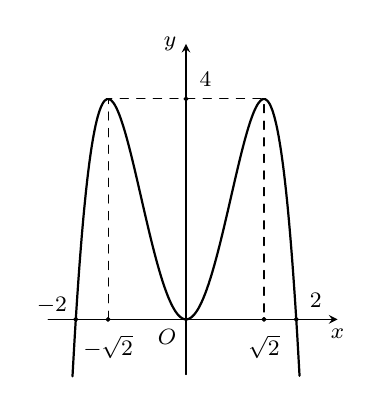
\begin{tikzpicture}[>=stealth,line join=round,line cap=round,font=\footnotesize,scale=0.7]
			\draw[->] (-2.5,0)--(2.75,0) node[below]{$x$};
			\draw[->] (0,-1)--(0,5) node[left]{$y$};
			\fill[name=O] (0,0) circle (1pt) node[below left] {$O$}; 
			\draw[thick,color=black, smooth, samples=100, domain= -2.06:2.06] plot(\x,{-(\x)^4 + 4*(\x)^2}) node[left]{$ $};
			\pgfmathsetmacro{\can}{sqrt(2)}
			\foreach  \d/\g/\l in {{-2,0}/150/-2,{2,0}/45/2,{-\can,0}/-90/-\sqrt{2},{\can,0}/-90/\sqrt{2},{0,4}/45/4}
				\draw[fill=black] (\d) circle (1pt) +(\g:.5) node{$\l$};
			\draw[dashed] (-\can,0)|-(0,4)-|(\can,0);
		\end{tikzpicture}
	}
	\loigiai{
		Từ đồ thị, ta có $\max\limits_{[0;2]}f(x)=4$.
	}
\end{ex}

%Câu 12
\begin{ex}%[2D1Y3-1]
	[Sở Bắc Giang 2019]
	\immini{
	Cho hàm số $y=f(x)$ liên tục trên đoạn $[-1;3]$ và có đồ thị như hình vẽ. Gọi $M$, $m$ lần lượt là giá trị lớn nhất và giá trị nhỏ nhất của hàm số đã cho trên đoạn $[-1;3]$. Giá trị của $M+m$ là
	\choice
	{$2$}
	{$-6$}
	{$-5$}
	{\True $-2$}
	}{
		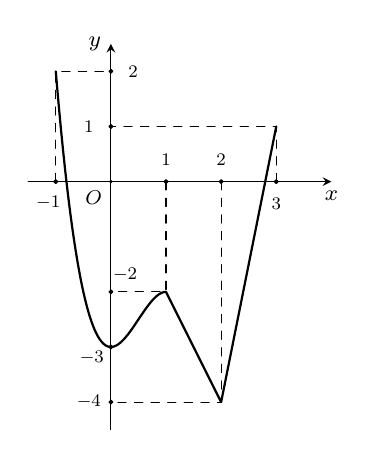
\begin{tikzpicture}[>=stealth,line join=round,line cap=round,font=\footnotesize,scale=0.7]
			\draw[->] (-1.5,0)--(4,0) node[below]{$x$};
			\draw[->] (0,-4.5)--(0,2.5) node[left]{$y$};
			\fill[name=O] (0,0) circle (1pt) node[below left,scale=0.9] {$O$}; 
			\draw[thick,color=black, smooth, samples=100, domain= -1:1] plot(\x,{-2*(\x)^3+ 3*(\x)^2-3}) node[left]{$ $};
			\draw[thick] (1,-2)--(2,-4)--(3,1);
			\foreach \d/\g/\l in {{-1,0}/-110/-1,{1,0}/90/1,{2,0}/90/2,{3,0}/-90/3,{0,-4}/180/-4,{0,-3}/-150/-3,{0,-2}/50/-2,{0,1}/180/1,{0,2}/0/2}
			 	\draw[fill=black] (\d) circle (1pt) +(\g:.4) node[scale=0.8]{$\l$}; 
			\draw[dashed] (-1,0)|-(0,2) (1,0)|-(0,-2) (2,0)|-(0,-4) (3,0)|-(0,1);
		\end{tikzpicture}
	}
	\loigiai{
		Từ đồ thị, ta có $M=\max\limits_{[-1;3]}f(x)=2$ và $m=\min\limits_{[-1;3]}f(x)=-4$.\\
		Vậy $M+m=-2$.
	}
\end{ex}

%Câu 13
\begin{ex}%[2D1Y3-1]
	[Sở Hà Nội 2019]
	Cho hàm số $y=f(x)$ có bảng biến thiên trên $[-5;7)$ như sau
	\begin{center}
		
\begin{tikzpicture}
			\tkzTabInit[nocadre=false,lgt=1.2,espcl=2.5,deltacl=.6]
			{$x$/0.6,$y'$/0.6,$y$/2}
			{$-5$,$1$,$7$}
			\tkzTabLine{,-,0,+,d}
			\tkzTabVar{+/$6$,-/$2$,+D/$9$}
		\end{tikzpicture}
	\end{center}
	Mệnh đề nào dưới đây đúng?
	\choice
	{$\min\limits_{[-5;7)}f(x)=6$}
	{\True $\min\limits_{[-5;7)}f(x)=2$}
	{$\min\limits_{[-5;7)}f(x)=9$}
	{$\min\limits_{[-5;7)}f(x)=6$}
	\loigiai{
		Từ bảng biến thiên, ta có $\min\limits_{[-5;7)}f(x)=2$.
	}
\end{ex}

%Câu 14
\begin{ex}%[2D1Y3-1]
	\immini{
	Cho hàm số $f(x)$ liên tục trên đoạn $[0;3]$ và có đồ thị như hình vẽ. Gọi $M$ và $m$ lần lượt là giá trị lớn nhất và giá trị nhỏ nhất của hàm số đã cho trên $[0;3]$. Giá trị của $M + m$ bằng
	\choice
	{$5$}
	{$3$}
	{$2$}
	{\True $1$}}
	{
		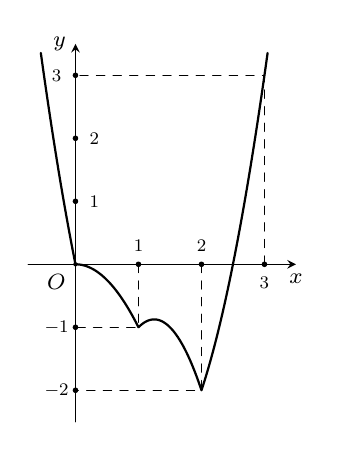
\begin{tikzpicture}[>=stealth,line join=round,line cap=round,font=\footnotesize,scale=0.8]
			\draw[->] (-0.75,0)--(3.5,0) node[below]{$x$};
			\draw[->] (0,-2.5)--(0,3.5) node[left]{$y$};
			\fill[name=O] (0,0) circle (1pt) node[below left] {$O$}; 
			\draw[thick,color=black, smooth, samples=100, domain= -0.55:0] plot(\x,{2*(\x)^2 - 5*(\x)});
			\draw[thick,color=black, smooth, samples=100, domain= 0:1] plot(\x,{-(\x)^2});
			\draw[thick,color=black, smooth, samples=100, domain= 1:2] plot(\x,{-2*(\x)^2 + 5*(\x) -4});
			\draw[thick,color=black, smooth, samples=100, domain= 2:3.05] plot(\x,{2*(\x)^2 - 5*(\x)});

			\foreach \d/\g/\l in {{1,0}/90/1,{2,0}/90/2,{3,0}/-90/3,{0,-2}/180/-2,{0,-1}/180/-1,{0,1}/0/1,{0,2}/0/2,{0,3}/180/3}
				\draw[fill=black] (\d) circle (1pt) +(\g:.3) node[scale=0.8]{$\l$};
			\draw[dashed] (1,0)|-(0,-1) (2,0)|-(0,-2) (3,0)|-(0,3);
		\end{tikzpicture}
	}
	\loigiai{
		Từ đồ thị hàm số, ta có $M=\max\limits_{[0;3]}f(x)=3$ và $m=\min\limits_{[0;3]}f(x)=-2$.\\
		Vậy $M+m = 1$.
	}
\end{ex}

%Câu 15
\begin{ex}%[2D1Y3-1]
	[Chuyên Lê Quý Đôn - Điện Biên 2019]
	\immini{
		Cho hàm số $y=f(x)$ liên tục trên đoạn $[-2;6]$ và có đồ thị như hình vẽ. Gọi $M$ và $m$ lần lượt là giá trị lớn nhất và nhỏ nhất của hàm số đã cho trên đoạn $[-2;6]$. Giá trị của $M-m$ bằng
		\choice
		{\True $9$}
		{$-8$}
		{$-9$}
		{$8$}
	}{
		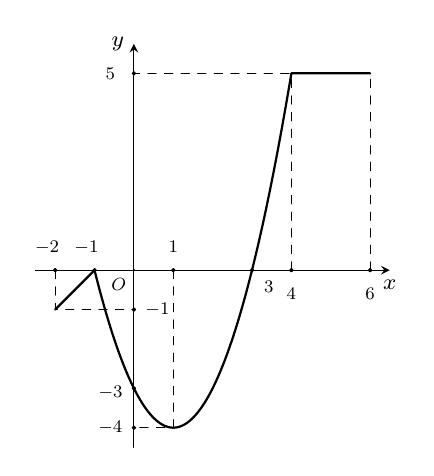
\begin{tikzpicture}[>=stealth,line join=round,line cap=round,font=\footnotesize,scale=0.5]
			\draw[->] (-2.5,0)--(6.5,0) node[below]{$x$};
			\draw[->] (0,-4.5)--(0,5.75) node[left]{$y$};
			\fill[name=O] (0,0) circle (1pt) node[below left,scale=0.8] {$O$}; 
			\draw[thick,color=black, smooth, samples=100, domain= -1:4] plot(\x,{((\x)-1)^2 -4}) node[left]{$ $};
			\draw[thick] (-2,-1)--(-1,0) (4,5)--(6,5);
			\foreach \d/\g/\l in {{-2,0}/110/-2,{-1,0}/110/-1,{1,0}/90/1,{3,0}/-45/3,{4,0}/-90/4,{6,0}/-90/6,{0,-4}/180/-4,{0,-3}/-170/-3,{0,-1}/0/-1,{0,5}/180/5}
				\draw[fill=black] (\d) circle (1.2pt) +(\g:.6) node[scale=0.8]{$\l$};
			\draw[dashed] (-2,0)|-(0,-1) (1,0)|-(0,-4) (4,0)|-(0,5) (6,0)--(6,5);
		\end{tikzpicture}
	}
	\loigiai{
		Từ đồ thị, ta có $M=\max\limits_{[-2;6]}f(x)=5$ và $m=\min\limits_{[-2;6]}f(x)=-4$.\\
		Vậy $M-m=9$.
	}
\end{ex}

%Câu 17
\begin{ex}%[2D1Y3-1]
	[THPT Ngô Sĩ Liên - Bắc Giang 2019]
	Cho hàm số $y=f(x)$ có bảng xét dấu đạo hàm như sau
	\begin{center}
		
\begin{tikzpicture}
			\tkzTabInit[nocadre=false,lgt=1.2,espcl=2,deltacl=.6]
			{$x$/0.6,$y'$/0.8}
			{$-\infty$,$-1$,$0$,$1$,$+\infty$}
			\tkzTabLine{,-,d,-,0,+,0,-,}
		\end{tikzpicture}
	\end{center}
	Mệnh đề nào sau đây đúng?
	\choice
	{$\max\limits_{(-1;1]}f(x)=f(0)$}
	{\True $\max\limits_{(0;+\infty)}f(x)=f(1)$}
	{$\min\limits_{(-\infty;-1)}f(x) = f(-1)$}
	{$\min\limits_{(-1;+\infty)}f(x) = f(0)$}
	\loigiai{
		Mệnh đề đúng là $\min\limits_{(0;+\infty)}f(x)=f(1)$.
	}
\end{ex}

\begin{dang}{Xác định giá trị lớn nhất - giá trị nhỏ nhất của hàm số trên đoạn từ công thức của hàm số}
\end{dang}

%Câu 1
\begin{ex}%[2D1Y3-1]
	[Đề minh họa 2020 Lần 1]
	Giá trị lớn nhất của hàm số $f(x)=-x^4 + 12x^2 +1$ trên đoạn $[-1;2]$ bằng
	\choice
	{$1$}
	{$37$}
	{\True $33$}
	{$12$}
	\loigiai{
	Ta có $f'(x)=-4x^3 + 24x=-4x\left(x^2-6\right)$.\\
	$f'(x)=0\Leftrightarrow \hoac{&x=0\\&x=\sqrt{6}\quad(\text{loại})\\&x=-\sqrt{6}\quad(\text{loại}).}$\\
	Mặt khác, $f(-1)=12$, $f(2)=33$, $f(0)=1$.\\
	Suy ra $\max\limits_{[-1;2]}f(x)=f(2)=33$.	
	}
\end{ex}

%Câu 2
\begin{ex}%[2D1Y3-1]
	[Đề tham khảo 2022 Lần 2]
	Giá trị nhỏ nhất của hàm số $f(x)=x^4 -10x^2 +2$ trên đoạn $[-1;2]$ bằng
	\choice
	{$2$}
	{$-23$}
	{\True $-22$}
	{$-7$}
	\loigiai{
		Ta có $f'(x)=4x^3 -20x = 4x\left(x^2-5\right)$.\\
		$f'(x)=0\Leftrightarrow \hoac{&x=0\\&x=\sqrt{5}\quad(\text{loại})\\&x=-\sqrt{5}\quad (\text{loại}).}$\\
		Mặt khác, $f(-1)=-7$, $f(2)=-22$, $f(0)=2$.\\
		Suy ra $\min\limits_{[-1;2]}f(x)=f(2)=-22$.
	}
\end{ex}

%Câu 3
\begin{ex}%[2D1Y3-1]
	[Mã 101 - 2020 Lần 1]
	Giá trị nhỏ nhất của hàm số $f(x)=x^3-24x$ trên đoạn $[2;19]$ bằng
	\choice
	{$32\sqrt{2}$}
	{$-40$}
	{\True $-32\sqrt{2}$}
	{$-45$}
	\loigiai{
		Ta có $f'(x)=3x^2 -24$.\\
		$f'(x)=0\Leftrightarrow \hoac{&x=2\sqrt{2}\\&x=-2\sqrt{2}\quad(\text{loại}).}$\\
		Mặt khác $f(2)=-40$, $f(19)=6403$, $f\left(2\sqrt{2}\right)=-32\sqrt{2}$.\\
		Suy ra $\min\limits_{[2;19]}f(x)=f\left(2\sqrt{2}\right)=-32\sqrt{2}$.
	}
\end{ex}

%Câu 4
\begin{ex}%[2D1Y3-1]
	Giá trị nhỏ nhất của hàm số $f(x)=x^3 -21x$ trên đoạn $[2;19]$ bằng
	\choice
	{$-36$}
	{\True $-14\sqrt{7}$}
	{$14\sqrt{7}$}
	{$-34$}
	\loigiai{
		Ta có $f'(x)=3x^2 -21$.\\
		$f'(x)=0 \Leftrightarrow \hoac{&x=\sqrt{7}\\&x=-\sqrt{7}\quad(\text{loại}).}$\\
		Mặt khác, $f(2)=-34$, $f(19)=6460$, $f\left(\sqrt{7}\right)=-14\sqrt{7}$.\\
		Suy ra $\min\limits_{[2;19]}f(x)=f\left(\sqrt{7}\right)=-14\sqrt{7}$.
	}
\end{ex}

%Câu 5
\begin{ex}%[2D1Y3-1]
	Giá trị nhỏ nhất của hàm số $f(x)=x^3 - 30x$ trên đoạn $[2;19]$ bằng
	\choice
	{$20\sqrt{10}$}
	{$-63$}
	{\True $-20\sqrt{10}$}
	{$-52$}
	\loigiai{
		Ta có $f'(x)=3x^2 -30$.\\
		$f'(x)=0 \Leftrightarrow \hoac{&x=\sqrt{10}\\&x=-\sqrt{10}\quad(\text{loại}).}$\\
		Mặt khác, $f(2)=-52$, $f(19)=6289$, $f\left(\sqrt{10}\right)=-20\sqrt{10}$.\\
		Suy ra $\min\limits_{[2;19]}f(x)=f\left(\sqrt{10}\right)=-20\sqrt{10}$.
	}
\end{ex}

\begin{ex}%[2D1Y3-1]%Câu 6
	[Mã 104 - 2020 Lần 1] Giá trị nhỏ nhất của hàm số $f(x)=x^3-33 x$ trên đoạn $[2;19]$ bằng
	\choice
	{$-72$}
	{\True $-22 \sqrt{11}$}
	{$-58$}
	{$22 \sqrt{11}$}
	\loigiai{
		Ta có $f'(x)=3 x^2-33=0 \Leftrightarrow\left[\begin{array}{l}x=\sqrt{11}\in[2 ; 19] \\ x=-\sqrt{11}\notin[2 ; 19].\end{array}\right.$\\
		Khi đó ta có $f(2)=-58$, $f(\sqrt{11})=-22 \sqrt{11}, f(19)=6232$.\\ Vậy $f_{\min}=f(\sqrt{11})=-22 \sqrt{11}$.}
\end{ex}

\begin{ex}%[2D1Y3-1]%Câu 7
	[Mã 101 - 2020 Lần 2] Giá trị nhỏ nhất của hàm số $f(x)=x^4-10 x^2-4$ trên $[0 ; 9]$ bằng
	\choice
	{$-28$}
	{$-4$}
	{$-13$}
	{\True $-29$}
	\loigiai{
		Hàm số $y=f(x)$ liên tục trên $[0 ; 9]$.\\
		Có $f'(x)=4 x^3-20 x$, $f'(x)=0 \Leftrightarrow\left[\begin{array}{l}x=0 \\ x=\sqrt{5}\\ x=-\sqrt{5}\notin[0 ; 9].\end{array}\right.$\\
		Ta có $f(0)=-4, f(\sqrt{5})=-29, f(9)=5747$.\\
		Do đó $\min\limits_{[0 ; 9]}f(x)=f(\sqrt{5})=-29$.}
\end{ex}

\begin{ex}%[2D1Y3-1]%Câu 8
	[Mã 102 - 2020 Lần 2] Giá trị nhỏ nhất của hàm số $f(x)=x^4-12 x^2-4$ trên đoạn $[0 ; 9]$ bằng
	\choice
	{$-39$}
	{\True $-40$}
	{$-36$}
	{$-4$}
	\loigiai{
		Ta có: $f'(x)=4 x^3-24 x ; f'(x)=0 \Leftrightarrow\left[\begin{array}{l}x=0 \\ x=\pm \sqrt{6}.\end{array}\right.$\\
		Tính được: $f(0)=-4 ; f(9)=5585$ và $f(\sqrt{6})=-40$.\\
		Suy ra $\min\limits_{[0 ; 9]}f(x)=-40$.}
\end{ex}

\begin{ex}%[2D1Y3-1]%Câu 9
	[Mã 103 - 2020 Lần 2] Giá trị nhỏ nhất của hàm số $f(x)=x^4-10 x^2-2$ trên đoạn $[0 ; 9]$ bằng
	\choice
	{$-2$}
	{$-11$}
	{$-26$}
	{\True $-27$}
	\loigiai{
		Ta có $f'(x)=4 x^3-20 x$.
		$$
		\begin{aligned}
			& f'(x)=0 \Leftrightarrow 4 x^3-20 x=0 \Leftrightarrow\left[\begin{array}{l}
				x=0 \notin(0 ; 9) \\
				x=\sqrt{5}\in(0 ; 9) \\
				x=-\sqrt{5}\notin(0 ; 9).
			\end{array}\right. \\
			& f(0)=-2 ; f(\sqrt{5})=-27 ; f(9)=5749. \\
			& \text{Vậy}\min _{[0 ; 9]}f(x)=-27.
		\end{aligned}
		$$}
\end{ex}

\begin{ex}%[2D1Y3-1]%Câu 10
	[Mã 104 - 2020 Lần 2] Giá trị nhỏ nhất của hàm số $f(x)=x^4-12 x^2-1$ trên đoạn $[0 ; 9]$ bằng
	\choice
	{$-28$}
	{$-1$}
	{$-36$}
	{\True $-37$}
	\loigiai{
		Ta có $f'(x)=4 x^3-24 x$.
		$$
		\begin{aligned}
			& f'(x)=0 \Leftrightarrow 4 x^3-24 x=0 \Leftrightarrow\left[\begin{array}{l}
				x=0 \in[0 ; 9] \\
				x=\sqrt{6}\in[0 ; 9] \\
				x=-\sqrt{6}\notin[0 ; 9].
			\end{array}\right. \\
			& f(0)=-1, f(\sqrt{6})=-37, f(9)=5588.
		\end{aligned}
		$$}
\end{ex}

\begin{ex}%[2D1Y3-1]%Câu 11
	[Mã 102 - 2019] Giá trị nhỏ nhất của hàm số $f(x)=x^3-3 x+2$ trên đoạn $[-3 ; 3]$ bằng
	\choice
	{$0$ }
	{\True $-16$}
	{$20$ }
	{$4$ }
	\loigiai{
		\textbf{Cách 1:} Mode $7$, nhập $f(x)=x^3-3 x+2$. Start $-3$. End $3$. Step $1$.\\
		\textbf{Cách 2:} $f'(x)=3 x^2-3 . f'(x)=0 \Leftrightarrow x=\pm 1 \in[-3 ; 3]$.\\
		$f(-3)=-16 ; f(-1)=4 ; f(1)=0 ; f(3)=20$.\\
		Giá trị nhỏ nhất là $-16$.
	}
\end{ex}

\begin{ex}%[2D1Y3-1]%Câu 12
	[Mã 110 2017] Tìm giá trị lớn nhất $M$ của hàm số $y=x^4-2 x^2+3$ trên đoạn $[0 ; \sqrt{3}]$.
	\choice
	{\True $M=6$}
	{$M=1$}
	{$M=9$}
	{$M=8 \sqrt{3}$}
	\loigiai{
		Ta có: $y'=4 x^3-4 x=4 x\left(x^2-1\right)$
		$$
		y'=0 \Leftrightarrow 4 x\left(x^2-1\right)=0 \Leftrightarrow\left[\begin{array}{l}
			x=0 \\
			x=1 \\
			x=-1 \text{ (loại).}
		\end{array}\right.
		$$
		Ta có : $y(0)=3$; $y(1)=2$; $y(\sqrt{3})=6$.\\
		Vậy giá trị lớn nhất của hàm số $y=x^4-2 x^2+3$ trên đoạn $[0 ; \sqrt{3}]$ là $M=y(\sqrt{3})=6$.
	}
\end{ex}

\begin{ex}%[2D1Y3-1]%Câu 13
	[Đề Minh Họa 2017] Tìm giá trị nhỏ nhất của hàm số $y=\dfrac{x^2+3}{x-1}$ trên đoạn $[2 ; 4]$.
	\choice
	{$\min\limits_{[2 ; 4]}y=-3$}
	{$\min\limits_{[2 ; 4]}y=\dfrac{19}{3}$}
	{\True $\min\limits_{[2 ; 4]}y=6$}
	{$\min\limits_{[2 ; 4]}y=-2$}
	\loigiai{
		Tập xác định: $\mathscr{D}=\mathbb{R}\backslash\{1\}$.\\
		Hàm số $y=\dfrac{x^2+3}{x-1}$ xác định và liên tục trên đoạn $[2 ; 4]$.\\
		Ta có $y'=\dfrac{x^2-2 x-3}{(x-1)^2}; y'=0 \Leftrightarrow x^2-2 x-3=0 \Leftrightarrow x=3$ hoặc $x=-1$ (loại).\\
		Suy ra $y(2)=7$ ; $y(3)=6$ ; $y(4)=\dfrac{19}{3}$.\\
		Vậy $\min\limits_{[2 ; 4]}y=6$ tại $x=3$.}
\end{ex}

\begin{ex}%[2D1Y3-1]%Câu 14
	[Mã 103 - 2019] Giá trị lớn nhất của hàm số $f(x)=x^3-3 x$ trên đoạn [ $\left.-3 ; 3\right]$ bằng
	\choice
	{$-2$}
	{\True 18 }
	{2 }
	{$-18$}
	\loigiai{
		Ta có $y'=3 x^2-3=0 \Leftrightarrow x=\pm 1$.
		$$
		f(-3)=-18 ; f(-1)=2 ; f(1)=-2 ; f(3)=18.
		$$}
\end{ex}

\begin{ex}%[2D1Y3-1]%Câu 15
	[Mã 104 2018] Giá trị lớn nhất của hàm số $y=x^4-x^2+13$ trên đoạn $[-1 ; 2]$ bằng
	\choice
	{$85$}
	{$\dfrac{51}{4}$}
	{$13$}
	{\True $25$}
	\loigiai{
		$$
		\begin{aligned}
			& y=f(x)=x^4-x^2+13 \\
			& y'=4 x^3-2 x \\
			& y'=0 \Leftrightarrow\left[\begin{array}{l}
				x=0 \in[-1 ; 2] \\
				x=-\dfrac{1}{\sqrt{2}}\in[-1 ; 2] \\
				x=\dfrac{1}{\sqrt{2}}\in[-1 ; 2]
			\end{array}\right. \\
			& f(-1)=13 ; f(2)=25 ; f(0)=13 ; f\left(-\dfrac{1}{\sqrt{2}}\right)=\dfrac{51}{4}; f\left(\dfrac{1}{\sqrt{2}}\right)=\dfrac{51}{4}.
		\end{aligned}
		$$
		Giá trị lớn nhất của hàm số $y=x^4-x^2+13$ trên đoạn $[-1 ; 2]$ bằng $25$.}
\end{ex}

\begin{ex}%[2D1Y3-1]%Câu 16
	[Mã 104 2017] Tìm giá trị nhỏ nhất $m$ của hàm số $y=x^2+\dfrac{2}{x}$ trên đoạn $\left[\dfrac{1}{2}; 2\right]$.
	\choice
	{$m=5$}
	{\True $m=3$}
	{$m=\dfrac{17}{4}$}
	{$m=10$}
	\loigiai{
		Đặt $y=f(x)=x^2+\dfrac{2}{x}$.\\
		Ta có $y'=2 x-\dfrac{2}{x^2}=\dfrac{2 x^3-2}{x^2}, y'=0 \Rightarrow x=1 \in\left[\dfrac{1}{2}; 2\right]$.\\
		Khi đó $f(1)=3, f\left(\dfrac{1}{2}\right)=\dfrac{17}{4}, f(2)=5$.\\
		Vậy $m=\min\limits_{\left[\frac{1}{2}; 2\right]}f(x)=f(1)=3$.}
\end{ex}

\begin{ex}%[2D1Y3-1]%Câu 17
	[Chuyên Bắc Ninh 2018] Tìm tập giá trị của hàm số $y=\sqrt{x-1}+\sqrt{9-x}$
	\choice
	{$T=[1 ; 9]$}
	{\True $T=[2 \sqrt{2}; 4]$}
	{$T=(1 ; 9)$}
	{$T=[0 ; 2 \sqrt{2}]$}
	\loigiai{
		Tập xác định: $\mathscr{D}=[1 ; 9]$
		$$
		\begin{aligned}
			& y'=\dfrac{1}{2 \sqrt{x-1}}-\dfrac{1}{2 \sqrt{9-x}}=0 \Leftrightarrow \sqrt{9-x}=\sqrt{x-1}\Leftrightarrow\left\{\begin{array}{l}
				x \geq 1 \\
				9-x=x-1
			\end{array}\Leftrightarrow x=5 .\right. \\
			& f(1)=f(9)=2 \sqrt{2}; f(5)=4
		\end{aligned}
		$$
		Vậy tập giá trị là $T=[2 \sqrt{2}; 4]$.}
\end{ex}

\begin{ex}%[2D1Y3-1]%Câu 18
	[Mã 123 2017] Tìm giá trị nhỏ nhất $m$ của hàm số $y=x^3-7 x^2+11 x-2$ trên đoạn $[0 ; 2]$.
	\choice
	{$m=3$}
	{$m=0$}
	{\True $m=-2$}
	{$m=11$}
	\loigiai{
		Xét hàm số trên đoạn $[0 ; 2]$.\\
		Ta có $y'=3 x^2-14 x+11$ suy ra $y'=0 \Leftrightarrow x=1$.\\
		Tính $f(0)=-2 ; f(1)=3, f(2)=0$.\\
		Suy ra $\min\limits_{[0 ; 2]}f(x)=f(0)=-2=m$.}
\end{ex}

\begin{ex}%[2D1Y3-1]%Câu 19
	[Mã 101 2018] Giá trị lớn nhất của hàm số $y=x^4-4 x^2+9$ trên đoạn $[-2 ; 3]$ bằng
	\choice
	{$201$}
	{$2$}
	{$9$}
	{\True $54$}
	\loigiai{
		$$
		y'=4 x^3-8 x ; y'=0 \Leftrightarrow\left[\begin{array}{l}
			x=0 \\
			x=\pm \sqrt{2}
		\end{array}.\right.
		$$
		Ta có $y(-2)=9$ ; $y(3)=54$ ; $y(0)=9$ ; $y(\pm \sqrt{2})=5$.\\
		Vậy $\max\limits_{[-2 ; 3]}y=54$.}
\end{ex}

\begin{ex}%[2D1Y3-1]%Câu 20
	[Đề Tham Khảo 2018] Giá trị lớn nhất của hàm số $f(x)=x^4-4 x^2+5$ trên đoạn $[-2 ; 3]$ bằng
	\choice
	{$122$}
	{\True $50$}
	{$5$}
	{$1$}
	\loigiai{
		$$
		\begin{aligned}
			& f'(x)=4 x^3-8 x=0 \Leftrightarrow\left[\begin{array}{l}
				x=0 \in[-2 ; 3] ;\\
				x=\pm \sqrt{2} \in[-2 ; 3].
			\end{array}\right. \\
			& f(0)=5 ; f(\pm \sqrt{2})=1 ; f(-2)=5 ; f(3)=50.
		\end{aligned}
		$$
		Vậy $\max\limits_{[-2 ; 3]}y=50$.
	}
\end{ex}

\begin{ex}%[2D1Y3-1]%Câu 21
	[Mã 105 2017] Tìm giá trị nhỏ nhất $m$ của hàm số $y=x^4-x^2+13$ trên đoạn $[-2 ; 3]$.
	\choice
	{$m=13$}
	{\True $m=\dfrac{51}{4}$}
	{$m=\dfrac{51}{2}$}
	{$m=\dfrac{49}{4}$}
	\loigiai{
		$$
		y'=4 x^3-2 x ; y'=0 \Leftrightarrow\left[\begin{array}{l}
			x=0 \in[-2 ; 3]; \\
			x=\pm \dfrac{1}{\sqrt{2}}\in[-2 ; 3].
		\end{array}\right.
		$$
		Tính $y(-2)=25$, $y(3)=85$, $y(0)=13$, $y\left(\pm \dfrac{1}{\sqrt{2}}\right)=\dfrac{51}{4}=12,75$.\\
		Kết luận: giá trị nhỏ nhất $m$ của hàm số là $m=\dfrac{51}{4}$.}
\end{ex}

\begin{ex}%[2D1Y3-1]%Câu 22
	[Mã 104 2019] Giá trị nhỏ nhất của hàm số $f(x)=x^3-3 x$ trên đoạn $[-3 ; 3]$ bằng
	\choice
	{\True $-18$}
	{$-2$}
	{$2$}
	{$18$}
	\loigiai{
		Ta có $f'(x)=3 x^2-3=0 \Leftrightarrow\left[\begin{array}{l}x=1 \\ x=-1\end{array}\right.$.\\
		Mà $f(-3)=-18 ; f(-1)=2 ; f(1)=-2 ; f(3)=18$.\\
		Vậy giá trị nhỏ nhất của hàm số $f(x)=x^3-3 x$ trên đoạn $[-3 ; 3]$ bằng $-18$.}
\end{ex}

\begin{ex}%[2D1Y3-1]%Câu 23
	[Mã 103 2018] Giá trị nhỏ nhất của hàm số $y=x^3+3 x^2$ trên đoạn $[-4 ;-1]$ bằng
	\choice
	{\True $-16$}
	{$0$}
	{$4$}
	{$-4$}
	\loigiai{
		Ta có $y'=3 x^2+6 x ; y'=0 \Rightarrow 3 x^2+6 x=0 \Leftrightarrow\left[\begin{array}{ll}x=0 & \notin[-4 ;-1] \\ x=-2 & \in[-4 ;-1]\end{array}\right.$.\\
		Khi đó $y(-4)=-16$ ; $y(-2)=4$ ; $y(-1)=2$.\\
		Vậy $\min _{[-4 ;-1]}y=-16$.}
\end{ex}

\begin{ex}%[2D1Y3-1]%Câu 24
	[Mã 102 2018] Giá trị nhỏ nhất của hàm số $y=x^3+2 x^2-7 x$ trên đoạn $[0 ; 4]$ bằng
	\choice
	{$-259$}
	{$68$}
	{$0$}
	{\True $-4$}
	\loigiai{
		Tập xác định $\mathscr{D}=\mathbb{R}$.\\
		Hàm số liên tục trên đoạn $[0 ; 4]$.
		Ta có $y'=3 x^2+4 x-7$
		$$
		\begin{aligned}
			& y'=0 \Leftrightarrow\left[\begin{array}{l}
				x=1 \in[0 ; 4] \\
				x=-\dfrac{7}{3}\notin[0 ; 4]
			\end{array}\right. \\
			& y(0)=0 ; y(1)=-4 ; y(4)=68 .
		\end{aligned}
		$$
		Vậy $\min\limits_{[0 ; 4]}y=-4$.}
\end{ex}

\begin{ex}%[2D1Y3-1]%Câu 25
	[Mã 101 - 2019] Giá trị lớn nhất của hàm số $f(x)=x^3-3 x+2$ trên đoạn $[-3 ; 3]$ là
	\choice
	{$4$}
	{$-16$}
	{\True $20$}
	{$0$}
	\loigiai{
		$f(x)=x^3-3 x+2$ tập xác định $\mathbb{R}$.
		$$
		\begin{aligned}
			& f'(x)=0 \Leftrightarrow 3 x^2-3=0 \Leftrightarrow x=\pm 1 \in[-3 ; 3] . \\
			& f(1)=0 ; f(-1)=4 ; f(3)=20 ; f(-3)=-16.
		\end{aligned}
		$$
		Từ đó suy ra $\max\limits_{[-3 ; 3]}f(x)=f(3)=20$.}
\end{ex}

\begin{ex}%[2D1Y3-1]%Câu 26
	[SGD Nam Định] Giá trị nhỏ nhất của hàm số $y=x^2+\dfrac{2}{x}$ trên đoạn $[2 ; 3]$ bằng
	\choice
	{$\dfrac{15}{2}$}
	{\True $5$}
	{$\dfrac{29}{3}$}
	{$3$}
	\loigiai{
		+ Ta có hàm số $y=f(x)=x^2+\dfrac{2}{x}$ xác định và liên tục trên $[2 ; 3]$.\\
		+ $y'=f'(x)=2 x-\dfrac{2}{x^2}; f'(x)=0 \Leftrightarrow x=1 \notin[2 ; 3]$ mà $f(2)=5, f(3)=\dfrac{29}{3}$.\\
		Vậy $\min\limits_{[2 ; 3]}y=5$ tại $x=2$.}
\end{ex}

\begin{ex}%[2D1Y3-1]%Câu 27
	[Sở Quảng Trị 2019] Tìm giá trị lớn nhất $M$ của hàm số $y=\dfrac{3 x-1}{x-3}$ trên đoạn $[0 ; 2]$
	\choice
	{\True $M=\dfrac{1}{3}$}
	{$M=-\dfrac{1}{3}$}
	{$M=5$}
	{$M=-5$}
	\loigiai{
		Trên đoạn $[0 ; 2]$ ta luôn có $y'=-\dfrac{8}{(x-3)^2}<0, \,\forall x \in(0 ; 2)$.\\
		Vì $y(0)=\dfrac{1}{3}$, $y(2)=-5$ nên $M=\max\limits_{[0 ; 2]}y=\dfrac{1}{3}$.
	}
\end{ex}

\begin{ex}%[2D1Y3-1]%Câu 28
	[Sở Nam Định-2019] Giá trị lớn nhất của hàm số $y=\sqrt{4-x^2}$ là
	\choice
	{\True $2$}
	{$0$}
	{$4$}
	{$1$}
	\loigiai{
		- Tập xác định: $D=[-2 ; 2]$.\\
		- Ta có: $y'=\dfrac{-x}{\sqrt{4-x^2}}\Rightarrow y'=0 \Leftrightarrow x=0 \in(-2 ; 2)$.\\
		- Ta có: $\left\{\begin{array}{l}y(-2)=y(2)=0 \\ y(0)=2\end{array}\Rightarrow \max\limits_{[-2 ; 2]}y=2.\right.$}
\end{ex}

\begin{ex}%[2D1Y3-1]%Câu 29
	[Đề Minh Họa 2021] Gọi $M$, $m$ lần lượt là giá trị lớn nhất, giá trị nhỏ nhất của hàm số $f(x)=x^4-2 x^2+3$ trên đoạn $[0 ; 2]$. Tổng $M+m$ bằng
	\choice
	{$11$}
	{$14$}
	{$5$}
	{\True $13$}
	\loigiai{
		Tập xác định: $\mathscr{D}=\mathbb{R}$.
		$$
		\begin{aligned}
			& f'(x)=4 x^3-4 x \\
			& f'(x)=0 \Leftrightarrow 4 x^3-4 x=0 \Leftrightarrow\left[\begin{array}{ll}
				x=0 & \in[0 ; 2] \\
				x=-1 & \notin[0 ; 2] \\
				x=1 & \in[0 ; 2]
			\end{array}\right. \\
			& f(0)=3 ; f(1)=2 ; f(2)=11 \\
			& \Rightarrow\left\{\begin{array}{l}
				M=11 \\
				m=2
			\end{array}\Rightarrow M+m=13 .\right.
		\end{aligned}
		$$}
\end{ex}

\begin{ex}%[2D1Y3-1]%Câu 30
	[Mã 101 - 2021 Lần 1] Trên đoạn $[0;3]$, hàm số $y=-x^3+3 x$ đạt giá trị lớn nhất tại điểm
	\choice
	{$x=0$}
	{$x=3$}
	{\True $x=1$}
	{$x=2$}
	\loigiai{
		Tập xác định: $\mathbb{R}$.\\
		$$
		\begin{aligned}
			& y'=-3 x^2+3 \\
			& y'=0 \Leftrightarrow-3 x^2+3=0 \Leftrightarrow\left[\begin{array}{l}
				x=1 \quad \in(0 ; 3) \\
				x=-1 \notin(0 ; 3)
			\end{array}\right. \\
			&
		\end{aligned}
		$$
		Ta có $y(0)=0 ; y(1)=2 ; y(3)=-18$.
		Vậy $\max\limits_{[0 ; 3]}y=y(1)=2$.}
\end{ex}

\begin{ex}%[2D1Y3-1]%Câu 31
	[Mã 103 - 2021 - Lần 1] Trên đoạn $[0 ; 3]$, hàm số $y=x^3-3 x+4$ đạt giá trị nhỏ nhất tại điểm
	\choice
	{\True $x=1$}
	{$x=0$}
	{$x=3$}
	{$x=2$}
	\loigiai{
		Ta có $y'=3 x^2-3$.\\
		$$
		y'=0 \Leftrightarrow\left[\begin{array}{l}
			x=1 \in[0 ; 3] \\
			x=-1 \notin[0 ; 3]
		\end{array}.\right.
		$$
		Lại có $y(0)=4 ; y(1)=2 ; y(3)=22$.
		Vậy $\min\limits_{[0 ; 3]}y=y(1)=2$}
\end{ex}

\begin{ex}%[2D1Y3-1]%Câu 32
	[Mã 102 - 2021 Lần 1] Trên đoạn $[-2 ; 1]$, hàm số $y=x^3-3 x^2-1$ đạt giá trị lớn nhất tại điểm
	\choice
	{$x=-2$}
	{\True $x=0$}
	{$x=-1$}
	{$x=1$}
	\loigiai{
		Ta có $y'=3 x^2-6 x \Rightarrow y'=0 \Leftrightarrow\left[\begin{array}{l}x=0 \\ x=2\end{array}\right.$.\\
		Ta đang xét trên đoạn $[-2 ; 1]$ nên loại $x=2$.\\
		Ta có $f'(-2)=-21 ; f'(0)=-1 ; f'(1)=-3$.\\
		Do đó giá trị lớn nhất của hàm số trên đoạn $[-2 ; 1]$ là $-1$, tại $x=0$.}
\end{ex}

\begin{ex}%[2D1Y3-1]%Câu 33
	[Mã 104 - 2021 Lần 1] Trên đoạn $[-1 ; 2]$, hàm số $y=x^3+3 x^2+1$ đạt giá trị nhỏ nhất tại điểm
	\choice
	{$x=2$}
	{\True $x=0$}
	{$x=-1$}
	{$x=1$}
	\loigiai{
		Xét hàm số $y=f(x)=x^3+3 x^2+1$.\\
		$\Rightarrow y'=f'(x)=3 x^2+6 x$.
		$+f'(x)=0 \Leftrightarrow 3 x^2+6 x=0 \Leftrightarrow\left[\begin{array}{l}x=0 \in[-1 ; 2] \\ x=-2 \notin[-1 ; 2]\end{array}\right.$.\\
		Ta có $f(-1)=3, f(0)=1$ và $f(2)=21$.\\
		Nên $\min\limits_{x \in[-1 ; 2]}f(x)=1$ khi $x=0$.}
\end{ex}

\begin{ex}%[2D1Y3-1]%Câu 34
	[Chuyên Bắc Ninh 2018] Tìm giá trị nhỏ nhất của hàm số $y=\sin ^2 x-4 \sin x-5$.
	\choice
	{$-20$}
	{\True $-8$}
	{$-9$}
	{$0$}
	\loigiai{
		Đặt $t=\sin x, t \in[-1 ; 1]$. Xét $f(t)=t^2-4 t-5, t \in[-1 ; 1]$.
		$f'(t)=2 t-4=0 \Leftrightarrow t=2 \notin[-1 ; 1]$.\\
		$f(1)=-8, f(-1)=0$.\\
		Ta thấy $\min\limits_{[-1 ; 1]}f(t)=f(1)=-8$.\\
		Vậy giá trị nhỏ nhất của hàm số là $-8$.}
\end{ex}

\begin{ex}%[2D1Y3-1]%Câu 35
	[THPT Hoa Lư A 2018] Gọi $m$, $M$ lần lượt là giá trị nhỏ nhất và giá trị lớn nhất của hàm số $f(x)=\dfrac{1}{2}x-\sqrt{x+1}$ trên đoạn $[0 ; 3]$. Tính tổng $S=2 m+3 M$.
	\choice
	{\True $S=-\dfrac{7}{2}$}
	{$S=-\dfrac{3}{2}$}
	{$-3$}
	{$S=4$}
	\loigiai{
		Ta có: $f'(x)=\dfrac{1}{2}-\dfrac{1}{2 \sqrt{x+1}}=\dfrac{\sqrt{x+1}-1}{2 \sqrt{x+1}}$, cho $f'(x)=0 \Rightarrow \sqrt{x+1}=1 \Leftrightarrow x=0 \in[0 ; 3]$.\\
		Khi đó: $f(0)=-1, f(3)=-\dfrac{1}{2}$ nên $m=-1$ và $M=-\dfrac{1}{2}$.\\
		Vậy $S=2 m+3 M=-\dfrac{7}{2}$.}
\end{ex}

\begin{ex}%[2D1Y3-1]%Câu 36
	[Chuyên ĐHSPHN - 2018] Tìm giá trị lớn nhất của hàm số $f(x)=\sin x+\cos 2 x$ trên $[0 ; \pi]$ là
	\choice
	{\True $\dfrac{9}{8}$}
	{$\dfrac{5}{4}$}
	{$2$}
	{$1$}
	\loigiai{
		$$
		f(x)=\sin x+\cos 2 x=\sin x+1-2 \sin ^2 x
		$$
		Đặt $\sin x=t \quad(0 \leq t \leq 1)$.
		$$
		\begin{aligned}
			& f(t)=-2 t^2+t+1, f'(t)=-4 t+1 \\
			& f'(t)=0 \Leftrightarrow t=\dfrac{1}{4}\\
			& f(0)=1, f(1)=0, f\left(\dfrac{1}{4}\right)=\dfrac{9}{8}\\
			& \text{Vậy}\max\limits_{[0 ; 1]}f(x)=\dfrac{9}{8}.
		\end{aligned}
		$$}
\end{ex}

\begin{ex}%[2D1Y3-1]%Câu 37
	[THPT Hà Huy Tập - 2018] Giá trị lớn nhất của hàm số $y=2 \cos x-\dfrac{4}{3}\cos ^3 x$ trên $[0 ; \pi]$ là
	\choice
	{$\dfrac{2}{3}$}
	{$\dfrac{10}{3}$}
	{\True $\dfrac{2 \sqrt{2}}{3}$}
	{$0$}
	\loigiai{
		Đặt: $t=\cos x \Rightarrow t \in[-1 ; 1] \Rightarrow y=2 t-\dfrac{4}{3}t^3$.
		$$
		y'=2-4 t^2 \quad y'=0 \Leftrightarrow\left[\begin{array}{l}
			x=\dfrac{-1}{\sqrt{2}}\in[-1 ; 1] \\
			x=\dfrac{1}{\sqrt{2}}\in[-1 ; 1]
		\end{array}.\right.
		$$
		Tính: $y(-1)=\dfrac{-2}{3}, y\left(\dfrac{-1}{\sqrt{2}}\right)=\dfrac{-2 \sqrt{2}}{3}, y\left(\dfrac{1}{\sqrt{2}}\right)=\dfrac{2 \sqrt{2}}{3}, y(1)=\dfrac{2}{3}$.\\
		Vậy: $\max\limits_{[0 ; \pi]}y=\dfrac{2 \sqrt{2}}{3}$}
\end{ex}

\begin{ex}%[2D1Y3-1]%Câu 38
	Gọi $M$, $m$ lần lượt là giá trị lớn nhất và giá trị nhỏ nhất của hàm số $y=\dfrac{3 \sin x+2}{\sin x+1}$ trên đoạn $\left[0 ; \dfrac{\pi}{2}\right]$ . Khi đó giá trị của $M^2+m^2$ là
	\choice
	{$\dfrac{31}{2}$}
	{$\dfrac{11}{2}$}
	{\True $\dfrac{41}{4}$}
	{$\dfrac{61}{4}$}
	\loigiai{
		Đặt $t=\sin x, t \in[0 ; 1]$.\\
		Xét hàm $f(t)=\dfrac{3 t+2}{t+1}$ liên tục trên đoạn $[0 ; 1]$ có $f'(t)=\dfrac{1}{(t+1)^2}>0, t \in[0 ; 1]$.\\
		Suy ra hàm số đồng biến trên $[0 ; 1]$.
		$$
		\begin{aligned}
			& \Rightarrow M=\operatorname{Max}_{[0 ; 1]}f(t)=f(1)=\dfrac{5}{2}\text{và}m=\underset{[0 ; 1]}{\operatorname{Min}}f(t)=f(0)=2 . \\
			& \text{Khi đó } M^2+m^2=\left(\dfrac{5}{2}\right)^2+2^2=\dfrac{41}{4}.
		\end{aligned}
		$$}
\end{ex}

\begin{ex}%[2D1Y3-1]%Câu 39
	[THPT Can Lộc - Hà Tĩnh - 2018] Cho hàm số $y=\dfrac{\sin x+1}{\sin ^2 x+\sin x+1}$. Gọi $M$ là giá trị lớn nhất và $m$ là giá trị nhỏ nhất của hàm số đã cho. Chọn mệnh đề đúng.
	\choice
	{$M=m+\dfrac{3}{2}$}
	{$M=\dfrac{3}{2}m$}
	{\True $M=m+1$}
	{$M=m+\dfrac{2}{3}$}
	\loigiai{
		Đặt $\sin x=t,(-1 \leq t \leq 1)$ ta được $y=\dfrac{t+1}{t^2+t+1}$.\\
		Xét hàm số $y=\dfrac{t+1}{t^2+t+1}$ trên đoạn $[-1 ; 1]$ ta có $y'=\dfrac{-t^2-2 t}{\left(t^2+t+1\right)^2}$.\\
		Giải phương trình $y'=0 \Leftrightarrow-t^2-2 t=0 \Leftrightarrow\left[\begin{array}{l}t=0 \text{ (thỏa mãn) } \\ t=-2 \text{ (loại) }. \end{array}\right.$.\\
		Vì $y(-1)=0$ ; $y(0)=1$ ; $y(1)=\dfrac{2}{3}$ nên
		$$
		\max\limits_{[-1 ; 1]}y=y(0)=1 \Rightarrow M=1 ; \min\limits_{[-1 ; 1]}y=y(-1)=0 \Rightarrow m=0.
		$$
		Vậy $M=m+1$.}
\end{ex}

\begin{ex}%[2D1Y3-1]%Câu 40
	[Đề minh họa 2022] Trên đoạn $[1 ; 5]$, hàm số $y=x+\dfrac{4}{x}$ đạt giá trị nhỏ nhất tại điểm
	\choice
	{$x=5$}
	{\True $x=2$}
	{$x=1$}
	{$x=4$}
	\loigiai{
		Hàm số $y=f(x)=x+\dfrac{4}{x}$ xác định trên $[1 ; 5]$.
		$$
		\begin{aligned}
			& f'(x)=1-\dfrac{4}{x^2}=\dfrac{x^2-4}{x^2}\\
			& f'(x)=0 \Leftrightarrow x^2-4=0 \Leftrightarrow\left[\begin{array}{l}
				x=2 \in[1 ; 5] \\
				x=-2 \notin[1 ; 5]
			\end{array}\right. \\
			& f'(1)=5 ; f(2)=4 ; f(5)=\dfrac{29}{5}.
		\end{aligned}
		$$
		Suy ra, hàm số đạt giá trị nhỏ nhất tại $x=2$.}
\end{ex}

\begin{ex}%[2D1Y3-1]%Câu 41
	[Mã 101-2022] Giá trị lớn nhất của hàm số $f(x)=x^3-3 x^2-9 x+10$ trên đoạn $[-2 ; 2]$ bằng
	\choice
	{$-12$}
	{$10$ }
	{\True $15$}
	{$-1$}
	\loigiai{
		Xét hàm số $f(x)=x^3-3 x^2-9 x+10$ trên đoạn $[-2 ; 2]$.
		$$
		\begin{aligned}
			& \Rightarrow f'(x)=3 x^2-6 x-9 \text{.}\\
			& f'(x)=0 \Leftrightarrow 3 x^2-6 x-9=0 \Leftrightarrow\left[\begin{array}{ll}
				x=-1 & \in[-2 ; 2] \\
				x=3 & \notin[-2 ; 2]
			\end{array}.\right. \\
			&
		\end{aligned}
		$$
		Ta có:
		$$
		f(-2)=8 ; f(-1)=15 ; f(2)=-12.
		$$
		Vậy giá trị lớn nhất của hàm số $f(x)=x^3-3 x^2-9 x+10$ trên đoạn $[-2 ; 2]$ bằng $15$.}
\end{ex}

\begin{dang}{Xác định giá trị lớn nhất - giá trị nhỏ nhất của hàm số trên khoảng $(a;b)$}
\end{dang}

\begin{ex}%[2D1Y3-1]%Câu 1
	[Đề Tham Khảo 2017] Tính giá trị nhỏ nhất của hàm số $y=3 x+\dfrac{4}{x^2}$ trên khoảng $(0 ;+\infty)$.
	\choice
	{$\min\limits_{(0 ;+\infty)}y=\dfrac{33}{5}$}
	{$\min\limits_{(0 ;+\infty)}y=2 \sqrt[3]{9}$}
	{\True $\min\limits_{(0 ;+\infty)}y=3 \sqrt[3]{9}$}
	{$\min\limits_{(0 ;+\infty)}y=7$}
	\loigiai{
		Cách 1:
		$$
		y=3 x+\dfrac{4}{x^2}=\dfrac{3 x}{2}+\dfrac{3 x}{2}+\dfrac{4}{x^2}\geq 3 \sqrt[3]{\dfrac{3 x}{2}\cdot \dfrac{3 x}{2}\cdot \dfrac{4}{x^2}}=3 \sqrt[3]{9}
		$$
		Dấu " =" xảy ra khi $\dfrac{3 x}{2}=\dfrac{4}{x^2}\Leftrightarrow x=\sqrt[3]{\dfrac{8}{3}}$.\\
		Vậy $\min\limits_{(0 ;+\infty)}y=3 \sqrt[3]{9}$.\\
		Cách 2:
		Xét hàm số $y=3 x+\dfrac{4}{x^2}$ trên khoảng $(0 ;+\infty)$.\\
		Ta có $y=3 x+\dfrac{4}{x^2}\Rightarrow y'=3-\dfrac{8}{x^3}$.\\
		Cho $y'=0 \Leftrightarrow \dfrac{8}{x^3}=3 \Leftrightarrow x^3=\dfrac{8}{3}\Leftrightarrow x=\sqrt[3]{\dfrac{8}{3}}$.\\
		Bảng biến thiên:
		\begin{center}
			
\begin{tikzpicture}
			\tkzTabInit[nocadre=false,lgt=1.2,espcl=2.5,deltacl=0.6]
			{$x$/0.8,$y'$/0.6,$y$/2}
			{$0$ ,$\sqrt[3]{\frac{8}{3}}$ ,$+\infty$}
			\tkzTabLine{,-,0,+,}
			\tkzTabVar{+/$ $,-/$3\sqrt[3]{9}$,+/$ $}
			\end{tikzpicture}
		\end{center}
		$$
		\Rightarrow \min\limits_{(0 ;+\infty)}y=y\left(\sqrt[3]{\dfrac{8}{3}}\right)=3 \sqrt[3]{9}.
		$$}
\end{ex}

\begin{ex}%[2D1Y3-1]%Câu 2
	Gọi $m$ là giá trị nhỏ nhất của hàm số $y=x-1+\dfrac{4}{x-1}$ trên khoảng $(1 ;+\infty)$. Tìm $m$ ?
	\choice
	{$m=5$}
	{\True $m=4$}
	{$m=2$}
	{$m=3$}
	\loigiai{
		Tập xác định $\mathscr{D}=R \backslash\{1\}$.\\
		$$
		y'=\dfrac{x^2-2 x-3}{(x-1)^2}, y'=0 \Leftrightarrow\left[\begin{array}{l}
			x=-1 \\
			x=3
		\end{array}\right. \text{.}
		$$
		Bảng biến thiên:
		\begin{center}
			
\begin{tikzpicture}
				\tkzTabInit[nocadre=false,lgt=1.2,espcl=2.5,deltacl=0.6]
				{$x$/0.6,$y'$/0.6,$y$/2}
				{$1$ ,$3$ ,$+\infty$}
				\tkzTabLine{,-,0,+,}
				\tkzTabVar{+/$+\infty$,-/$4$,+/$+\infty$}
			\end{tikzpicture}
		\end{center}
		$$
		\Rightarrow m=\min\limits_{(1 ;+\infty)}y=4 \text{ khi } x=3.
		$$}
\end{ex}

\begin{ex}%[2D1Y3-1]%Câu 3
	[THPT Minh Châu Hưng Yên 2019] Giá trị nhỏ nhất của hàm số $y=x-5+\dfrac{1}{x}$ trên khoảng $(0 ;+\infty)$ bằng bao nhiêu?
	\choice
	{$0$}
	{$-1$}
	{\True $-3$}
	{$-2$}
	\loigiai{
		Áp dụng bất đẳng thức Cô-si ta có:
		$$
		y=x+\dfrac{1}{x}-5 \geq 2 \sqrt{x \cdot \dfrac{1}{x}}-5=-3
		$$
		Dấu bằng xảy ra khi $x=\dfrac{1}{x}\Leftrightarrow x^2=1 \Leftrightarrow x=1$ (vì $x>0$ ).\\
		Vậy $\min\limits_{(0 ;+\infty)}y=-3$}
\end{ex}

\begin{ex}%[2D1Y3-1]%Câu 4
	(Chuyên Lương Thế Vinh Đồng Nai 2019) Gọi $m$ là giá trị nhở nhất của hàm số $y=x+\dfrac{4}{x}$ trên khoảng $(0 ;+\infty)$. Tìm $m$
	\choice
	{\True $m=4$}
	{$m=2$}
	{$m=1$}
	{$m=3$}
	\loigiai{
		$$
		\begin{aligned}
			& y'=1-\dfrac{4}{x^2}\\
			& y'=0 \Leftrightarrow x=\pm 2 ; \quad x=2 \in(0 ;+\infty) .
		\end{aligned}
		$$
		Bảng biến thiên:
		\begin{center}
			
\begin{tikzpicture}
				\tkzTabInit[nocadre=false,lgt=1.2,espcl=2.5,deltacl=0.6]
				{$x$/0.6,$y'$/0.6,$y$/2}
				{$0$ ,$2$ ,$+\infty$}
				\tkzTabLine{,-,0,+,}
				\tkzTabVar{+/$+\infty$,-/$4$,+/$+\infty$}
			\end{tikzpicture}
		\end{center}
		Suy ra giá trị nhỏ nhất của hàm số bằng $y(2)=4 \Rightarrow m=4$.}
\end{ex}

\begin{ex}%[2D1Y3-1]%Câu 5
	[Chuyên Bắc Giang 2019] Giá trị nhỏ nhất của hàm số $f(x)=x+\dfrac{1}{x}$ trên nửa khoảng $[2 ;+\infty)$ là
	\choice
	{$2$}
	{\True $\dfrac{5}{2}$}
	{$0$}
	{$\dfrac{7}{2}$}
	\loigiai{
		Áp dụng bất đẳng thức Cô-si, ta được: $f(x)=x+\dfrac{1}{x}=\dfrac{3 x}{4}+\dfrac{x}{4}+\dfrac{1}{x}\geq \dfrac{3 \cdot 2}{4}+2 \sqrt{\dfrac{x}{4}}\cdot \dfrac{1}{x}=\dfrac{5}{2}$.\\
		Dấu bằng xảy ra khi $x=2$.}
\end{ex}

\begin{ex}%[2D1Y3-1]%Câu 6
	Gọi $m$ là giá trị nhỏ nhất của hàm số $y=x+\dfrac{4}{x}$ trên khoảng $(0 ;+\infty)$. Tìm $m$.
	\choice
	{$m=3$}
	{\True $m=4$}
	{$m=2$}
	{$m=1$}
	\loigiai{
	\textbf{Cách 1:}
		Hàm số $y=x+\dfrac{4}{x}$ liên tục và xác định trên $(0 ;+\infty)$.\\
		Ta có $y'=1-\dfrac{4}{x^2}=\dfrac{x^2-4}{x^2}\Rightarrow y'=0 \Leftrightarrow\left[\begin{array}{l}x=2 \in(0 ;+\infty) \\ x=-2 \notin(0 ;+\infty)\end{array}\right.$.\\
		Bảng biến thiên:
		\begin{center}
			
\begin{tikzpicture}
				\tkzTabInit[nocadre=false,lgt=1.2,espcl=2.5,deltacl=0.6]
				{$x$/0.6,$y'$/0.6,$y$/2}
				{$0$ ,$2$ ,$+\infty$}
				\tkzTabLine{,-,0,+,}
				\tkzTabVar{+/$+\infty$,-/$4$,+/$+\infty$}
			\end{tikzpicture}
		\end{center}
		Vậy giá trị nhỏ nhất là $m=4$ khi $x=2$.\\
	\textbf{Cách 2:}
		Với $x \in(0 ;+\infty) \Rightarrow x>0 ; \dfrac{4}{x}>0$.\\
		Áp dụng bất đẳng thức Cô-si ta có: $x+\dfrac{4}{x}\geq 2 \sqrt{x \cdot \dfrac{4}{x}}=4$.\\
		Dấu bằng xảy ra khi và chỉ khi $\left\{\begin{array}{l}x>0 \\ x=\dfrac{4}{x}\end{array}\Leftrightarrow x=2\right.$.\\
		Vậy $m=4$ khi $x=2$.}
\end{ex}

\begin{ex}%[2D1Y3-1]%Câu 7
	Giá trị nhỏ nhất của hàm số $y=\sqrt{4-x}+\sqrt{3}$ trên tập xác định của nó là
	\choice
	{$2+\sqrt{3}$}
	{$2 \sqrt{3}$}
	{$0$}
	{\True $\sqrt{3}$}
	\loigiai{
		Tập xác định của hàm số là: $\mathscr{D}=(-\infty ; 4]$.\\
		Ta có $y'=\dfrac{-1}{2 \sqrt{4-x}}<0, \forall x \in \mathscr{D}$.\\
		Bảng biến thiên:
		\begin{center}
			
\begin{tikzpicture}
				\tkzTabInit[nocadre=false,lgt=1.2,espcl=3.5,deltacl=0.6]
				{$x$/0.6,$y'$/0.6,$y$/2}
				{$-\infty$, $4$}
				\tkzTabLine{,-,}
				\tkzTabVar{+/$+\infty$,-/$\sqrt{3}$}
			\end{tikzpicture}
		\end{center}
		Từ bảng biến thiên suy ra $\min\limits_{(-\infty ; 4]}y=\sqrt{3}$ khi $x=4$.}
\end{ex}

\begin{ex}%[2D1Y3-1]%Câu 8
	Với giá trị nào của $x$ thì hàm số $y=x^2+\dfrac{1}{x}$ đạt giá trị nhỏ nhất trên khoảng $(0 ;+\infty)$ ?
	\choice
	{$\dfrac{3}{\sqrt[3]{4}}$}
	{$\dfrac{1}{\sqrt{2}}$}
	{$1$}
	{\True $\dfrac{1}{\sqrt[3]{2}}$}
	\loigiai{
		Tập xác định $\mathscr{D}=\mathbb{R}\setminus\{0\}$.\\
		$$
		y'=2 x-\dfrac{1}{x^2}, y'=0 \Leftrightarrow x=\dfrac{1}{\sqrt[3]{2}}.
		$$
		\begin{center}
			\begin{tikzpicture}
				\tikzset{double style/.append style={double distance=2pt}}
				\tkzTabInit[nocadre=false,lgt=1.2,espcl=2.5,deltacl=0.5]
				{$x$/1,$y'$/0.6,$y$/2}
				{$-\infty$,$0$,$\frac{1}{\sqrt[3]{2}}$,$+\infty$}
				\tkzTabLine{,-,d,-,0,+,}
				\path
				(N12)node[below](A){$+\infty$}
				(N23)node[above left](B){$-\infty$}
				(N22)node[below right](C){$+\infty$}
				($(N32)!0.75!(N33)$)node(D){$\sqrt[3]{2}+\frac{1}{\sqrt[3]{4}}$}
				(N42)node[below](E){$+\infty$};
				\draw[double distance=2pt](N22)--(N23);
				\foreach\x/\y in{A/B,C/D,D/E}\draw[-latex](\x)--(\y);
			\end{tikzpicture}
		\end{center}
		Dựa vào $\mathrm{BBT}$ thì $x=\dfrac{1}{\sqrt[3]{2}}$ hàm số đạt giá trị nhỏ nhất trên $(0 ;+\infty)$.}
\end{ex}

\begin{ex}%[2D1Y3-1]%Câu 9
	Giá trị nhỏ nhất của hàm số $y=x+\dfrac{2}{x}-(1+\sqrt{2})^2$ trên khoảng $(0 ;+\infty)$
	\choice
	{không tồn tại}
	{\True $-3$}
	{$-1+\sqrt{2}$}
	{$0$}
	\loigiai{
		Hàm số xác định và liên tục trên khoảng $(0 ;+\infty)$.
		$$
		\begin{aligned}
			& y'=1-\dfrac{2}{x^2}=\dfrac{x^2-2}{x^2}. \\
			& y'=0 \Leftrightarrow\left[\begin{array}{l}
				x=\sqrt{2}\\
				x=-\sqrt{2}
			\end{array}.\right.
		\end{aligned}
		$$
		Bảng biến thiên:
		\begin{center}
			
\begin{tikzpicture}
				\tkzTabInit[nocadre=false,lgt=1.2,espcl=2.5,deltacl=0.6]
				{$x$/0.6,$y'$/0.6,$y$/2}
				{$0$ ,$\sqrt{2}$ ,$+\infty$}
				\tkzTabLine{,-,0,+,}
				\tkzTabVar{+/$+\infty$,-/$-3$,+/$+\infty$}
			\end{tikzpicture}
		\end{center}
		Vậy $\min\limits_{(0 ;+\infty)}y=f(\sqrt{2})=-3$.}
\end{ex}

\begin{ex}%[2D1Y3-1]%Câu 10
	Cho hàm số $f(x)=\dfrac{\sqrt{x^2-1}}{x-2}$ với $x$ thuộc $\mathscr{D}=(-\infty ;-1] \cup\left[1 ; \dfrac{3}{2}\right]$. Mệnh đề nào dưới đây đúng?
	\choice
	{\True $\max\limits_\mathscr{D} f(x)=0 ; \min\limits_\mathscr{D} f(x)=-\sqrt{5}$}
	{$\max\limits_\mathscr{D} f(x)=0 ;$ không tồn tại $\min\limits_\mathscr{D} f(x)$}
	{$\max\limits_\mathscr{D} f(x)=0 ; \min\limits_\mathscr{D} f(x)=-1$}
	{$\min\limits_\mathscr{D} f(x)=0$; không tồn tại $\max\limits_\mathscr{D} f(x)$}
	\loigiai{
		Hàm số xác định và liên tục trên $\mathscr{D}=-\infty ;-1 \cup\left[1 ; \dfrac{3}{2}\right]$.
		$$
		f'x=\dfrac{-2 x+1}{x-2^2 \sqrt{x^2-1}}; f'(x)=0 \Leftrightarrow x=\dfrac{1}{2}\notin \mathscr{D}.
		$$
		\begin{center}	
			
\begin{tikzpicture}
				\tikzset{double style/.append style={double distance=2pt}}
				\tkzTabInit[nocadre=false,lgt=1.2,espcl=2.5,deltacl=0.6]
				{$x$/0.9,$f'(x)$/0.6,$f(x)$/2}
				{$-\infty$,$-1$,$1$,$\frac{3}{2}$}
				\tkzTabLine{,+,d, h ,d ,-,}
				\tkzTabVar{-/$-1$,+DH/$0$/,D+/$0$,-/$\sqrt{5}$}
			\end{tikzpicture}
		\end{center}
		Vậy $\max\limits_\mathscr{D} f(x)=0 ; \min\limits_\mathscr{D} f(x)=-\sqrt{5}$}
\end{ex}

\begin{ex}%[2D1Y3-1]%Câu 11
	[Cụm liên trường Hải Phòng 2019] Mệnh đề nào sau đây là đúng về hàm số $y=\dfrac{x+1}{\sqrt{x^2+5}}$ trên tập xác định của nó.
	\choice
	{Hàm số không có giá trị lớn nhất và không có giá trị nhỏ nhất}
	{Hàm số không có giá trị lớn nhất và có giá trị nhỏ nhất}
	{Hàm số có giá trị lớn nhất và giá trị nhỏ nhất}
	{\True Hàm số có giá trị lớn nhất và không có giá trị nhỏ nhất}
	\loigiai{
		Tập xác định: $\mathscr{D}=\mathbb{R}$.
		$$
		\begin{aligned}
			& y'=\dfrac{\sqrt{x^2+5}-x+1 \dfrac{2 x}{2 \sqrt{x^2+5}}}{x^2+5}=\dfrac{x^2+5-x^2-x}{\sqrt{x^2+5}x^2+5}=\dfrac{5-x}{\sqrt{x^2+5}x^2+5}. \\
			& y'=0 \Leftrightarrow \dfrac{5-x}{\sqrt{x^2+5}x^2+5}=0 \Leftrightarrow 5-x=0 \Leftrightarrow x=5.
		\end{aligned}
		$$
		Bảng biến thiên:
		\begin{center}
			
\begin{tikzpicture}
				\tkzTabInit[nocadre=false,lgt=1.2,espcl=2.5,deltacl=0.6]
				{$x$/0.6,$y'$/0.6,$y$/2}
				{$-\infty$ ,$5$ ,$+\infty$}
				\tkzTabLine{,+,0,-,}
				\tkzTabVar{-/$-1$,+/$\dfrac{\sqrt{30}}{5}$,-/$-1$}
			\end{tikzpicture}
		\end{center}
		Từ bảng biến thiên có $\max\limits_{\mathbb{R}}y=y(5) = \dfrac{\sqrt{30}}{5}$ khi $x=5$.\\
		Hàm số $y=\dfrac{x+1}{\sqrt{x^2+5}}$ không có giá trị nhỏ nhất.\\
		Vậy hàm số có giá trị lớn nhất và không có giá trị nhỏ nhất.}
\end{ex}

\Closesolutionfile{ans}
\indapan{10}{ans/CD3/Muc_5_6}